\documentclass[12pt,a4paper]{article}
%\usepackage{ctex}
\usepackage{amsmath,amscd,amsbsy,amssymb,latexsym,url,bm,amsthm}
\usepackage{epsfig,graphicx,subfigure}
\usepackage{enumitem,balance}
\usepackage{wrapfig}
\usepackage{mathrsfs,euscript}
\usepackage[usenames]{xcolor}
\usepackage{hyperref}
\usepackage[vlined,ruled,linesnumbered]{algorithm2e}
\usepackage{array}
\hypersetup{colorlinks=true,linkcolor=black}

\newtheorem{theorem}{Theorem}
\newtheorem{lemma}[theorem]{Lemma}
\newtheorem{proposition}[theorem]{Proposition}
\newtheorem{corollary}[theorem]{Corollary}
\newtheorem{exercise}{Exercise}
\newtheorem*{solution}{Solution}
\newtheorem{definition}{Definition}
\theoremstyle{definition}

\renewcommand{\thefootnote}{\fnsymbol{footnote}}

\newcommand{\postscript}[2]
 {\setlength{\epsfxsize}{#2\hsize}
  \centerline{\epsfbox{#1}}}

\renewcommand{\baselinestretch}{1.0}

\setlength{\oddsidemargin}{-0.365in}
\setlength{\evensidemargin}{-0.365in}
\setlength{\topmargin}{-0.3in}
\setlength{\headheight}{0in}
\setlength{\headsep}{0in}
\setlength{\textheight}{10.1in}
\setlength{\textwidth}{7in}
\makeatletter \renewenvironment{proof}[1][Proof] {\par\pushQED{\qed}\normalfont\topsep6\p@\@plus6\p@\relax\trivlist\item[\hskip\labelsep\bfseries#1\@addpunct{.}]\ignorespaces}{\popQED\endtrivlist\@endpefalse} \makeatother
\makeatletter
\renewenvironment{solution}[1][Solution] {\par\pushQED{\qed}\normalfont\topsep6\p@\@plus6\p@\relax\trivlist\item[\hskip\labelsep\bfseries#1\@addpunct{.}]\ignorespaces}{\popQED\endtrivlist\@endpefalse} \makeatother

\begin{document}
\noindent

%========================================================================
\noindent\framebox[\linewidth]{\shortstack[c]{
\Large{\textbf{Lab07-Amortized Analysis}}\vspace{1mm}\\
CS214-Algorithm and Complexity, Xiaofeng Gao \& Lei Wang, Spring 2021.}}
\begin{center}
\footnotesize{\color{red}$*$ If there is any problem, please contact TA Yihao Xie. }

\footnotesize{\color{blue}$*$ Name:BeichenYu  \quad Student ID:519030910245 \quad Email:polarisybc@sjtu.edu.cn}
\end{center}
\begin{enumerate}
	\item Suppose we perform a sequence of n operations on a data structure in which the $i$ th 		operation costs $i$ if $i$ is an exact power of 2, and 1 otherwise. Use an accounting method to determine the amortized cost per operation.
	
	\begin{solution}
	Assume a cost of \$3 for each operation. The operation from $(2^i+1)$th to $(2^{i+1}-1)$th costs \$1 actually, so we have a total credit of \$$2\times ((2^{i+1}-1) - (2^i+1) + 1) =$ \$$ 2^{i+1} - 2$. Together with the \$3 of the $2^{i+1}$th operation, we have a total of \$$2^{i+1} + 1$ to pay for the actual cost of \$$2^{i+1}$.  Thus, for any operation we have nonnegative credit. So the amortized cost per operation is $O(1)$.
	
	\end{solution}

	\item Consider an ordinary \textbf{binary min-heap} data structure with $n$ elements supporting
the instructions \textsc{Insert} and \textsc{Extract-Min} in $O(\log n)$ worst-case time. Give a
potential function $\Phi$ such that the amortized cost of \textsc{Insert} is $O(\log n)$ and the
amortized cost of \textsc{Extract-Min} is $O(1)$, and show that it works.
	
	\begin{solution}
	
	Let $D_i$ be the heap after the i-th operation. Assume that there are $n_i$ elements in $D_i$. Assume each \textsc{Insert} and \textsc{Extract-Min} operation takes $k\log n$ time at most.
	
	Define that $\Phi(D_i) = kn_i \log n_i$ if $n_i > 0$, and if the heap is empty, $\Phi(D_i) = 0$.
	
	If the i-th operation is an \textsc{Insert}, we have $n_i = n_{i-1} + 1$. 
	
	If the i-th operation inserts into an empty heap, we have $n_{i-1} = 0$ and $n_i = 1$, so we have:
	\begin{align*}
	\hat{c_i} &= c_i + \Phi(D_i) - \Phi(D_{i-1})\\
	&\leqslant k\log 1 + k\log 1 - 0\\
	&= 0
	\end{align*}
	
	If the i-th operation inserts into an non-empty heap, we have:
	\begin{align*}
	\hat{c_i} &= c_i + \Phi(D_i) - \Phi(D_{i-1})\\
	&\leqslant k\log n_i + kn_i\log n_i - k(n_{i-1})\log n_{i-1}\\
	&= k\log n_i + kn_i\log n_i - k(n_i-1)\log (n_i-1)\\
	&= k\log n_i + kn_i\log n_i - kn_i\log (n_i-1)+k\log (n_i-1)\\
	&\leqslant 2k\log n_i + kn_i \log \frac{n_i}{n_i - 1}\\
	&\leqslant 2k\log n_i + kn_i (\frac{n_i}{n_i - 1}-1)\\
	&\leqslant 2k\log n_i + k\frac{n_i}{n_i - 1}\\
	&\leqslant 2k\log n_i + 2k\\
	&= O(\log n_i)
	\end{align*}
	
	
	If the i-th operation is an \textsc{Extract-Min}, we have $n_i = n_{i-1} - 1$. 
	
	If before the i-th operation, there is only one element in the heap,  we have:
	\begin{align*}
	\hat{c_i} &= c_i + \Phi(D_i) - \Phi(D_{i-1})\\
	&\leqslant k\log 1 + 0 - k\log 1\\
	&= 0
	\end{align*}
	
	If before the i-th operation, there are more than one elements in the heap,  we have:
	\begin{align*}
	\hat{c_i} &= c_i + \Phi(D_i) - \Phi(D_{i-1})\\
	&\leqslant k\log n_{i-1} + kn_i\log n_i - k(n_{i-1})\log n_{i-1}\\
	&= k\log n_{i-1}  + k (n_{i-1} - 1)\log (n_{i-1} - 1) - kn_{i-1}\log n_{i-1}\\
	&= k\log \frac{n_{i-1}}{n_{i-1}-1}+kn_{i-1}\log \frac{n_{i-1}-1}{n_{i-1}}\\
	&\leqslant 	k\log \frac{n_{i-1}}{n_{i-1}-1}\\
	&\leqslant k\log2\\
	&=O(1)
	\end{align*}
	\end{solution}
	\item Assume we have a set of arrays $A_0, A_1, A_2,\cdots$, where the $i^{th}$ array $A_i$ has a length of $2^i$. Whenever an element is inserted into the arrays, we always intend to insert it into $A_0$. If $A_0$ is full then we pop the element in $A_0$ off and insert it with the new element into $A_{1}$. (Thus, if $A_{i}$ is already full, we recursively pop all its members off and insert them with the elements popped from $A_0,...,A_{i-1}$ and the new element into $A_{i+1}$ until we find an empty array to store the elements.) An illustrative example is shown in Figure \ref{Fig-MultiArray}. Inserting or popping an element take $O(1)$ time.

	\begin{figure}[!htbp]
	\centering
	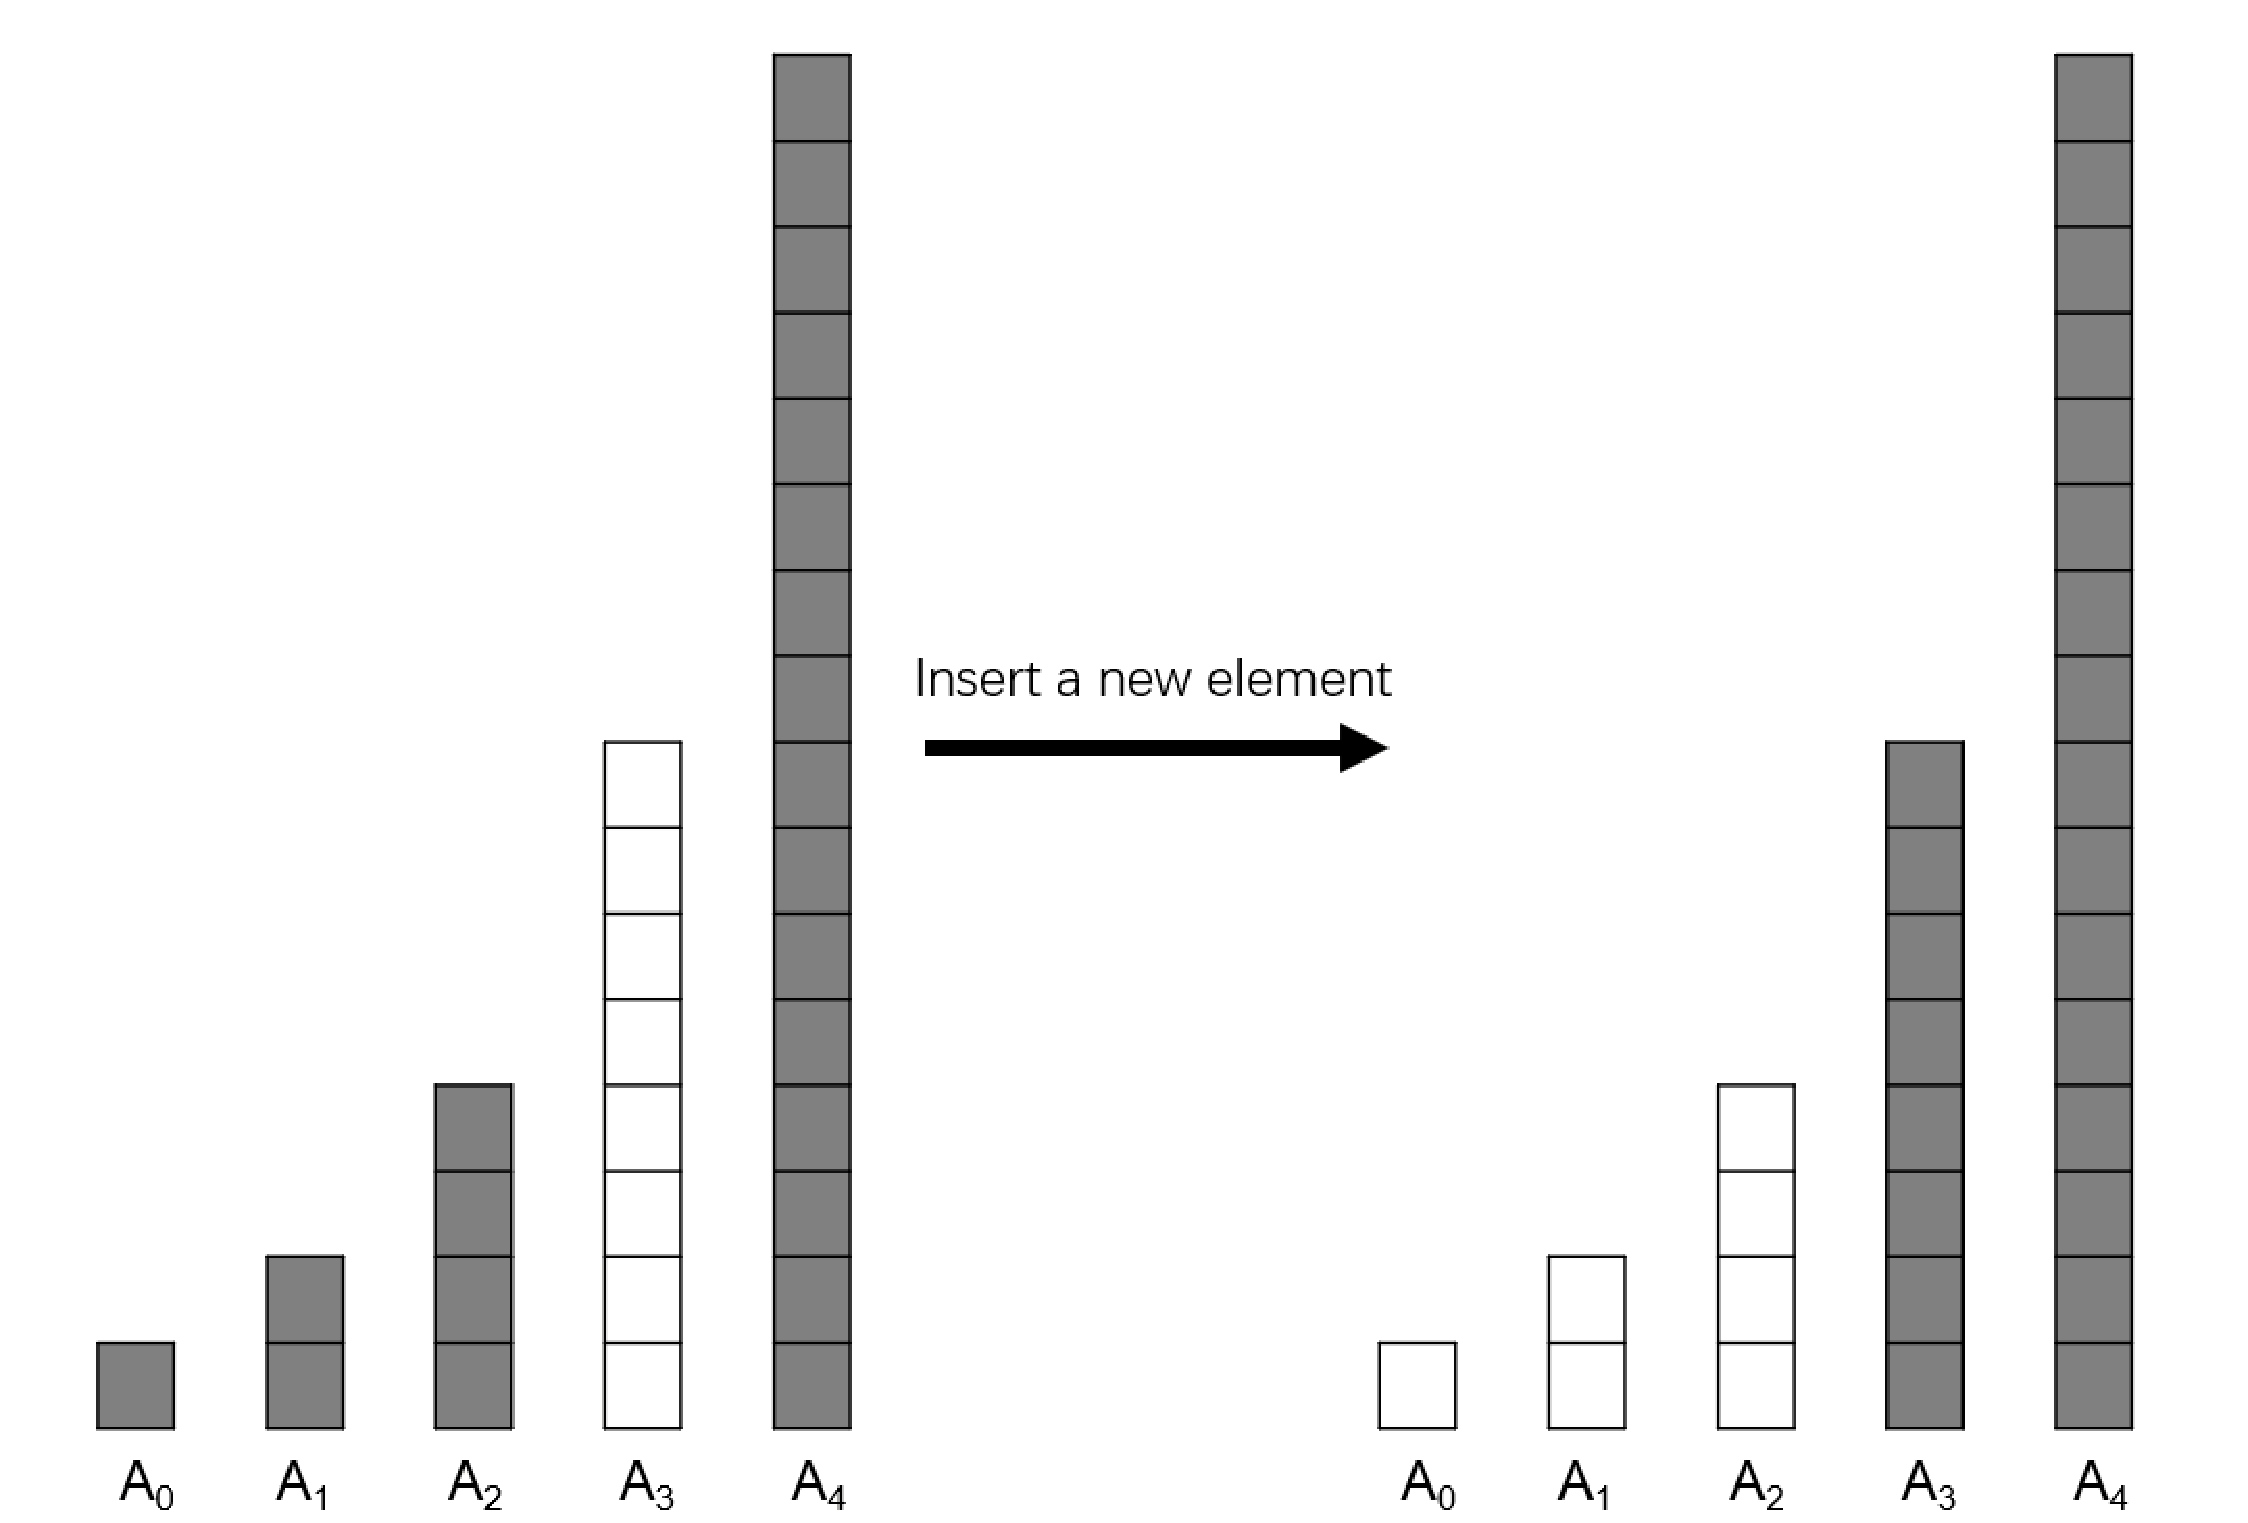
\includegraphics[width=0.5\textwidth]{Fig-MultiArray.pdf}
	\caption{An example of making room for one new element in the set of arrays.}
	\label{Fig-MultiArray}
	\end{figure}

    \begin{enumerate}
        \item In the worst case, how long does it take to add a new element into the set of arrays containing $n$ elements?
        \item Prove that the amortized cost of adding an element is $O(\log n)$ by \emph{Aggregation Analysis}.
        \item If each array $A_i$ is required to be sorted but elements in different arrays have no relationship with each other, how long does it take in the worst case to search an element in the arrays containing $n$ elements? 
\item What is the amortized cost of adding an element in the case of (c) if the comparison between two elements also takes $O(1)$ time?
    \end{enumerate}
	\begin{solution}

\begin{enumerate}
\item In the worst case, every nonempty array is full. To add a new element, we have to move all the elements to the next array. As there are already $n$ elements, to move all these elements, we need $O(n)$ time. 
\item First, to push a new element into the arrays, we need $O(1)$ time.

 Second, to move the $i^{th}$ array to the next one,we need to pop and push for $O(2^{i-1})$ times, so the time complexity is $2O(2^{i-1}) = O(2^i)$.
 
 Third, in the first $n$ operations, the times of moving the $i^{th}$ array is: 
 $$[\frac{n-\sum^{i-1}_{k=0}2^{k}}{2^{i-1}}] = [\frac{n - 2^i + 1}{2^{i-1}}] = [\frac{n+1}{2^{i-1}}]-2$$
 
 Therefore, the time of first $n$ pushing operations is:
 \begin{align*}
 T(n) &= n+\sum_{k=1}^{[\log_{2} (n+1)]}2^{k}([\frac{n+1}{2^{k-1}}]-2)\\
 &= n+\sum_{k=1}^{[\log_{2} (n+1)]}(2[n+1]-2^{k+1})\\
 &= n+2[n+1][\log_{2} (n+1)]-4(2^{[\log_{2} (n+1)]}-1)\\
 &= O(n\log n) 
 \end{align*}
 
 So the amortized cost of adding an element is: $$O(\frac{n\log n}{n}) = O(\log n)$$

\item In the $i^{th}$ array $A_{i}$ with $2^{i-1}$ elements, using the binary search, the worst case is to find the needed element in the last turn or the needed element is not in that array. That take $\log_{2} 2^{i-1} = i -1$ time. So in the worst case in total, it takes:
\begin{align*}
T_{worst} &=  \sum_{k=1}^{[\log_{2} (n+1)]} (k-1)\\
&= \frac{[\log_{2} (n+1)]([\log_{2} (n+1)]-1)}{2}\\
&= O(\log^2 n)
\end{align*}

\item Compare with (b), to push a new element into the arrays, we need still $O(1)$ time. When moving the full arrays, we need to make a merge sort. If we merge two arrays with size $m$ and $n$, the time complexity is $O(m+n)$. So we can merge the arrays from small to big. So merge $A_1,A_2,\cdots A_i$ the time complexity is at most $2^i$. So moving the $i^{th}$ array needs $2^{i+1}$ time. 

So we have:
 \begin{align*}
 T(n) &= n+\sum_{k=1}^{[\log_{2} (n+1)]}2^{k+1}([\frac{n+1}{2^{k-1}}]-2)\\
 &= n+\sum_{k=1}^{[\log_{2} (n+1)]}(4[n+1]-2^{k+2})\\
 &= n+4[n+1][\log_{2} (n+1)]-8(2^{[\log_{2} (n+1)]}-1)\\
 &= O(n\log n) 
 \end{align*}

\end{enumerate}
 So the amortized cost of adding an element is: $$O(\frac{n\log n}{n}) = O(\log n)$$
\end{solution}
\end{enumerate}


\textbf{Remark:} Please include your .pdf, .tex files for uploading with standard file names.


%========================================================================
\end{document}
